\documentclass[a4paper,12pt]{article}
%\usepackage[utf8x]{inputenc}
\usepackage{fontspec}
\usepackage{xeCJK}
\usepackage{xcolor,colortbl}
\setCJKmainfont{DFMing-Md-HK-BF.ttf}
%% Language and font encodings
%\usepackage[english]{babel}
%\usepackage[T1]{fontenc}
\usepackage{minted}
\usepackage{indentfirst}
%% Sets page size and margins
\usepackage[a4paper,top=2.5cm,bottom=2.5cm,left=2.5cm,right=2.5cm,marginparwidth=0.5cm]{geometry}
\usepackage{hyperref}
\usepackage{comment}
\renewcommand{\figurename}{圖}
\renewcommand{\figureautorefname}{圖}
\renewcommand{\tablename}{表}
\renewcommand{\tableautorefname}{表}
\setlength{\parindent}{2em}
\setlength{\parskip}{0.5em}
\renewcommand{\baselinestretch}{1.4}
%\usepackage[explicit]{titlesec}
%\usepackage{tikz}
%\usetikzlibrary{shapes,shadows,calc}
%\usepackage{lipsum}

%\definecolor{visgreen}{rgb}{0.733, 0.776, 0}

% the tikz picture that will be used for the title formatting
% \SecTitle{<signal direction>}{<node anchor>}{<node horiz, shift>}{<node x position>}{#5}
% the fifth argument will be used by \titleformat to write the section title using #1
%\newcommand\SecTitle[5]{%
%\begin{tikzpicture}[overlay,every node/.style={signal, draw, text=white, signal to=nowhere}]
%  \node[visgreen,fill, signal to=#1, inner sep=0.5em,
%    text=white,font=\Large\sffamily,anchor=#2,
%    xshift=\the\dimexpr-\marginparwidth-\marginparsep-#3\relax] 
%    at (#4,0) {#5};
%\end{tikzpicture}%
%}
%\titleformat{name=\section,page=odd}
%{\normalfont}{}{0em}
%{\SecTitle{east}{west}{16pt}{0}{#1}}[\addvspace{4ex}]

%\titleformat{name=\section,page=even}
%{\normalfont\sffamily}{}{0em}
%{\SecTitle{west}{east}{14pt}{\paperwidth}{#1}}[\addvspace{4ex}]



%% Useful packages
%\usepackage{amsmath}
%\usepackage{graphicx}
%\usepackage[colorinlistoftodos]{todonotes}
\definecolor{bgc}{rgb}{0.95,0.95,0.95}
\definecolor{LightCyan}{rgb}{0.88,1,1}
%\usepackage[colorlinks=true, allcolors=blue]{hyperref}
%\usepackage{abstract}
\renewcommand{\abstractname}{}%}\large 摘要}
\newcommand{\cc}{C\texttt{++}}

\newminted{cpp}{xleftmargin=.8cm,linenos,baselinestretch=1.2,autogobble=true,tabsize=4,showtabs=false,frame=single,framesep=10pt}
\newminted[inside]{cpp}{tabsize=4,autogobble=true,baselinestretch=1.2}

\title{2017年程式設計先修暑期夏令營\\學生上課講義}
%\author{王佳盈 梁家萁 侯怡安 朱睿謙 巫鈺瑩 周身鴻}
\begin{document}
\maketitle
%\begin{abstract}
%\chapter{前言}
我喜歡寫程式,寫程式可以說是學習和電腦打交道的過程。在寫程式的過程中,會發現電腦可以說得上是一位忠實、公正,又極有耐心的朋友,這些特質電腦發揮得極其盡緻,世間的朋友很難比得上。首先它非常客觀公正,無論情況多麼撲朔迷離,它仍然會在其中依循既定的原則而行,絕沒有一絲一豪偏離軌道;也不管你的程式功力多麼高深,程式寫得多麼巨大華麗,對於那豪不起眼的一點小小錯誤,它也絕不會輕易地把你放過,這是它忠實、公正的特質。另外,不管你的程式能力多麼拙劣,永無止盡的在相同的小錯誤中周旋,它也絕不失去耐心,乃至發出一點點怒火,仍然保持著冷靜沈著,一再地把最忠實而相同的錯誤訊息反應給你,這樣的耐心幾乎無人能及。如果要說它的一些缺點,大概就是有點不盡人情,有時候迂腐得可以。

寫程式跟學習世間的技能,過程非常一致。一個人學習游泳,學習騎腳踏車,如果沒有真正下水或上路練習,而只是詳細閱讀教學手冊,要真正在水中得到游泳的樂趣,或者在路上騎乘的快感,那幾乎是不太可能的事。同樣地,一個學習寫程式的人,如果沒有真正上機練習,而光是閱讀程式教學的書籍,要真正具備寫作程式的能力,那也是非常困難的事情。初學游泳的人,總是要在水中嗆幾口水;初學騎腳踏車的人,也不免有不穩或摔倒的時候,這都是學習過程普遍發生的事情。相同地,初學程式的人,總會有弄不清頭緒,在不解的錯誤中周旋的時候,這是一種除錯和學習的過程,不用因此而灰心喪志,只要持續努力,慢慢會掌握寫程式的一些絕竅。

我因為喜歡寫程式,後來也有機會開始擔任C/\cc{}程式的教學。因為了解學習程式必須實際練習,所以也一直在尋找合適的學習資源。現在網路非常發達,資訊詳盡而多元,要找到一些學習資源並不太難,但是在尋找C/\cc{}的學習資源的過程中,發現大部份的學習工具和平台多是英語介面,對於國內很多學生來說,還是有一些不容易跨越的門檻。後來在尋覓的過程中,發現了銘傳大學謝育平老師所寫作的「瘋狂程設」,這個平台不僅完全使用中文,而且還可以把許多教學、作業和解題的過程融合在一個系統中,不僅對初學程式的人極有幫助,對於程式教學的老師來說,也提供非常有用的資源,可以達到事半功倍的效果。後來也承蒙謝老師的幫助,連續幾年開課,我都一直使用這個學習平台,作為教學的輔助資源。

「瘋狂程設」的平台中,提供了很多練習題目,可以讓學習程式的人練習,而老師也可以使用這個系統,不斷開發新的題目。對於剛入門的同學來說,「瘋狂程設」有一個程式練習廣場,裡面很有系統地提供一些基礎的題目,讓初學的人練習解題,漸次深入,這就好像玩遊戲過關斬將一樣,讓學習程式也可以變得很有樂趣。對於老手來說,這些題目可能不堪一擊,但對初學者來說,很多人經常卡關,面對題目不知所措,甚至充滿了挫折。這本書的內容,主要就是針對程式練習廣場的題目,提供詳盡的思惟過程和解題參考,可以作為初學者的破關攻略,也可以從中看到各種不同的解題技巧。

這本書能夠完成,還要特別感謝實驗室幾位研究生,包括梁家萁、侯怡安、朱睿謙、巫鈺瑩、以及周身鴻等人。我讓他們每個人先練習撰寫書中的一小部份章節,一方面他們可以練習,一方面我也可以減輕一些負擔,等他們寫完各章節之後,我再整體看過並做修改。所以這本書能夠完成,也要非常感謝這些同學的幫忙。

我希望這本書可以幫助到初學C/\cc{}程式的人,也希望提供給程式教學的老師作為教學的參考,減輕彼此教和學的負擔和困難,乃至達到事半功倍的效果。書中的內容,主要針對問題如何思考和解答來做說明,所以不是完整的教科書,很多C/\cc{}語言基本的概念,還是應該要參閱其他的書籍和資源。

另外,寫程式要有相對應的開發工具,在教學上,我習慣使用的整合開發環境是Code::Blocks,這是一套跨平台的自由軟體,功能實用而且豐富;而編譯程式用的編譯器則是使用mingw,這是gcc移植到Windows的版本,也可以說是非常普及而強大的編譯工具。讀者只要連到Code::Blocks的官網,可以直接下載內含mingw的Code::Blocks版本,非常便利。本書第一部份也會針對Code::Blocks的安裝以及瘋狂程設的使用做一些說明。

我必須再次強調,學習程式一定要自己思考和練習,如果只是光看而不練的話,實際遇到問題,還是做不出來的。因此同學在使用本書的時候,除了閱讀之外,也要花一些時間自己思考,並且實際上機練習解題,務求每一個步驟都充份了解和熟悉,這樣才能達到理想的功效。

對於本書的內容,如果有什麼修正建議或錯誤指正,還請不吝提供給我們作為修正的參考,連絡方式,可以寄信到\ \href{mailto:jywglady@gmail.com}{jywglady@gmail.com}\ 電子信箱,我們先在此感謝您的幫忙。最後敬祝大家學習愉快,一切平安吉祥。

\begin{flushright}
	王佳盈 寫於 2018/06
\end{flushright}

%\end{abstract}
\ \\ \\ \\ \\ \\
\begin{center}
	本課程獲教育部扎根高中職資訊科學教育計畫補助
\end{center} 
\newpage
這份講義,僅提供給同學作為學習參考之用,希望說可以幫助大家學習C/\cc{}程式語言。
講義的內容,主要針對問題如何思考和解答來做說明,所以不是完整的教科書,很多C/\cc{}語言基本的概念,還是應該要參閱其他的書籍和資源。

另外,寫程式要有相對應的開發工具,我們使用的整合開發環境是Code::Blocks,這是一套跨平台的自由軟體,而編譯程式用的編譯器是使用mingw,這是gcc移植到Windows的版本。另外為了方便學習,我們也使用「瘋狂程設」線上學習系統做為輔助的學習資源,瘋狂程設提供了一個很好的解題學習環境,對於學習程式語言可以提供一些幫助,所以講義也會針對Code::Blocks的安裝以及瘋狂程設的使用做一些說明。

基本上,學習程式一定要自己思考和練習,如果只是光看而不練的話,實際遇到問題,還是做不出來的。因此大家在使用這份講義的時候,除了閱讀之外,也要花一些時間自己思考,然後實際上機練習解題,務求每一個步驟都充份了解和熟悉,這樣才能達到理想的功效。

另外,這份講義還在修改階段,請自行參考使用,勿隨意流傳。如果有什麼修正的建議,可以提供給我們,感謝大家。連絡方式,可以當面說明,或者寄信到 \href{mailto:jywglady@gmail.com}{jywglady@gmail.com} 或 \href{mailto:dachurita@gmail.com}{dachurita@gmail.com}。

\newpage
\setcounter{tocdepth}{2}
\tableofcontents

\section{猜數字:幾A幾B(人猜)}

電腦選定一個沒有重複的三位數當作答案,使用者每猜一個數字,電腦會根據答案給出幾A幾B的提示。A表示位置正確的數的個數,B表示數字正確但位置錯誤的數的個數。

使用者根據提示一直猜,直到猜中為止。
\begin{figure}[H]
	\centering
	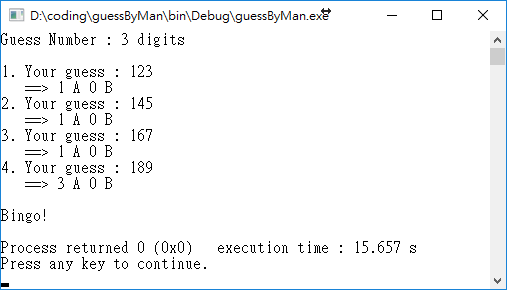
\includegraphics{fig/man}
\end{figure}
\subsection{解題思惟}

\subsubsection{程式流程:}
\begin{enumerate}
	\item 取得一個不重複的三位數。
	\item 讓使用者輸入猜的數字。
	\item 計算幾個A。
	\item 計算幾個B
	\item 若沒猜中,回到步驟2,猜中則結束程式。
\end{enumerate}

\subsubsection{函式說明:}
\begin{enumerate}
	\item int getRand3()
	
	此函數用來產生一個不重複的三位數。整數a, b, c分別是此三位數的百位、十位及個位數,一次只選定一個位數的值,每次使用$rand()\%10$來取得一個介於0-9之間的隨機亂數,若與其他位數的值相同,則重新取亂數,一直取到與其他位數不相等為止。最終取得的三位數是$(a*100+b*10+c)$。
	
	\item int countA(int guess, int ans)
	
	此函數用來計算幾個A。參數guess是使用者猜的數字,ans是答案。使用\%10分別取得guess及ans的個位數,比較兩數,若相等,則cnt++。比較完之後將guess及ans分別除以10。因為guess及ans是一個三位數,所以用for迴圈執行3次比較。最後輸出cnt即可知道猜中幾個A。
	
	\item int countB(int guess, int ans)
	
	此函數用來計算幾個B。將guess及ans的個位、十位及百位數分別存入陣列a及陣列b。使用雙重for迴圈掃描所有情況,若位置不同$(i != j)$且數字相同$(a[i] == b[j])$,則cnt++。最後輸出cnt即可知道猜中幾個B。
\end{enumerate}

\subsection{程式碼}
\begin{cppcode}
#include <iostream>
#include <cstdlib>
#include <ctime>

using namespace std;

int getRand3();
int countA(int guess, int ans);
int countB(int guess, int ans);

int main()
{
	int mynumber, yourguess, idx=1;
	cout << "Guess Number : 3 digits\n\n";
	mynumber = getRand3();
	do {
		cout << idx++ << ". Your guess : ";
		cin >> yourguess;
		int a = countA(mynumber, yourguess);
		int b = countB(mynumber, yourguess);
		cout << "   ==> " << a << " A " << b << " B" << endl;
	} while (yourguess != mynumber);
	cout << endl << "Bingo!" << endl;
	return 0;
}

int countA(int guess, int ans)
{
	int d1, d2, cnt=0;
	for (int i=0; i<3; i++) {
		d1 = guess % 10;
		d2 = ans % 10;
		if (d1==d2) cnt++;
		guess /= 10;
		ans /= 10;
	}
	return cnt;
}

int countB(int guess, int ans)
{
	int a[3], b[3], cnt=0;
	for (int i=0; i<3; i++) {
		a[i] = guess % 10;
		b[i] = ans % 10;
		guess /= 10;
		ans /= 10;
	}
	for (int i=0; i<3; i++) {
		for (int j=0; j<3; j++) {
			if (i!=j && a[i]==b[j]) cnt++;
		}
	}
	return cnt;
}

int getRand3()
{
	int a, b, c;
	srand(time(NULL));
	
	a = rand() % 10; // 0--9
	
	do {
		b = rand() % 10;
	} while (b==a);  // if b==a, re-choose b
	
	do {
		c = rand() % 10;
	} while (c==a || c==b);  // if c==a or c==b, re-choose c
	
	return a*100+b*10+c;
}
\end{cppcode}
\section{猜數字:幾A幾B(電腦猜)}

使用者選定一個沒有重複的三位數當作答案,電腦每猜一個數字,使用者就要根據答案給出幾A幾B的提示。A表示位置正確的數的個數,B表示數字正確但位置錯誤的數的個數。

電腦根據提示一直猜,直到猜中為止。
\begin{figure}[H]
	\centering
	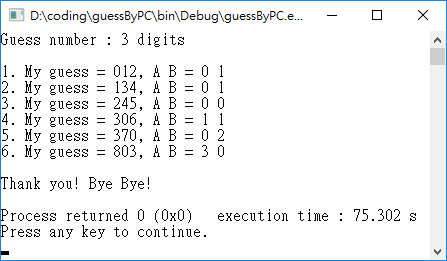
\includegraphics{fig/PC}
\end{figure}
\subsection{解題思惟}

\subsubsection{程式流程:}
\begin{enumerate}
	\item 初始化陣列,將不可能成為答案的元素設成0,其他設成1。
	\item 輸出一個可能的答案。
	\item 讓使用者輸入幾A幾B。
	\item 根據幾A幾B將不可能的答案剔除。
	\item 若沒猜中,回到步驟2,猜中則結束程式。
\end{enumerate}

\subsubsection{函式說明:}
\begin{enumerate}
	\item void initCandidates()
	
	此函數用來初始化陣列。在0-999的整數中,分別取出個位、十位及百位數。若三個數字有重複,則不可能成為答案,將此元素設為0,其他元素設為1。
	
	\item int validGuess()
	
	此函數選出電腦猜的數字。用for迴圈掃描陣列,若是可能的答案,則回傳。
	
	\item updateCandidates(int number, int ga, int gb)
	
	此函數用來更新陣列。用for迴圈掃描陣列,若是可能的答案,判斷是否符合幾A幾B,若不符合,則將此元素設為0。
\end{enumerate}

\subsection{程式碼}
\begin{cppcode}
#include <cstdio>

int candidates[1000];

void initCandidates();
int  validGuess();
void updateCandidates(int number, int ga, int gb);
int  countA(int guess, int ans);
int  countB(int guess, int ans);

int main()
{
	int guess, idx=1, a, b;
	
	initCandidates();
	printf("Guess number : 3 digits\n\n");
	do {
		guess = validGuess();
		printf("%d. My guess = %03d, A B = ", idx++, guess);
		scanf("%d%d", &a, &b);
		updateCandidates(guess, a, b);
	} while (a!=3 || b!=0);
	printf("\nThank you! Bye Bye!\n");
	
	return 0;
}

// init candidates, erase all number with same digit
void initCandidates()
{
	for (int n=0; n<1000; n++) {
		int a = n/100;       // a..
		int b = (n/10) % 10; // .b.
		int c = n % 10;      // ..c
		if (a==b || b==c || c==a) candidates[n]=0;
		else candidates[n]=1;
	}
}

int validGuess()
{
	for (int i=0; i<1000; i++) {
		if (candidates[i]) return i;
	}
	return -1; // No possible candidate
}

void updateCandidates(int number, int ga, int gb)
{
	for (int i=0; i<1000; i++) {
		if (candidates[i]) {
			if (ga != countA(number, i)) candidates[i] = 0;
			if (gb != countB(number, i)) candidates[i] = 0;
		}
	}
}

int countA(int guess, int ans)
{
	int d1, d2, cnt=0;
	for (int i=0; i<3; i++) {
		d1 = guess % 10;
		d2 = ans % 10;
		if (d1==d2) cnt++;
		guess /= 10;
		ans /= 10;
	}
	return cnt;
}

int countB(int guess, int ans)
{
	int a[3], b[3], cnt=0;
	for (int i=0; i<3; i++) {
		a[i] = guess % 10;
		b[i] = ans % 10;
		guess /= 10;
		ans /= 10;
	}
	for (int i=0; i<3; i++) {
		for (int j=0; j<3; j++) {
			if (i!=j && a[i]==b[j]) cnt++;
		}
	}
	return cnt;
}

\end{cppcode}

\end{document}
